\documentclass[a4paper, 11pt]{article}
\usepackage{amsmath}
\usepackage{graphicx}
\usepackage{geometry}
\usepackage{listings}
\usepackage{color}
\usepackage{cite}

\definecolor{dkgreen}{rgb}{0,0.6,0}
\definecolor{gray}{rgb}{0.5,0.5,0.5}
\definecolor{mauve}{rgb}{0.58,0,0.82}
\lstset{frame=shadowbox,
    language=Python,
    aboveskip=3mm,
    belowskip=3mm,
    showstringspaces=false,
    columns=flexible,
    basicstyle={\small\ttfamily},
    numbers=left,
    numberstyle=\tiny\color{gray},
    keywordstyle=\color{blue},
    commentstyle=\color{dkgreen},
    stringstyle=\color{mauve},
    breaklines=true,
    breakatwhitespace=true,
    tabsize=3
}
\usepackage[colorlinks,linkcolor=red]{hyperref}
\geometry{scale=0.8}

\title{	
\normalfont \normalsize
\textsc{School of Data and Computer Science, Sun Yat-sen University} \\ [25pt] %textsc small capital letters
\rule{\textwidth}{0.5pt} \\[0.4cm] % Thin top horizontal rule
\huge  Maze Problem\\ % The assignment title
\rule{\textwidth}{2pt} \\[0.5cm] % Thick bottom horizontal rule
\author{17341203 Yixin Zhang}
\date{\normalsize\today}
}

\begin{document}
\maketitle
\tableofcontents
\newpage
\section{Task}



\begin{itemize}
	\item Please solve the maze problem (i.e., find the shortest path from the start point to the finish point) by using BFS or DFS (Python or C++)
	\item The maze layout can be modeled as an array, and you can use the data file \texttt{MazeData.txt} if necessary.
	\item Please send \texttt{E01\_YourNumber.pdf} to \texttt{ai\_201901@foxmail.com}, you can certainly use \texttt{E01\_Maze.tex} as the \LaTeX template.
\end{itemize}

\begin{figure}[ht]
\centering
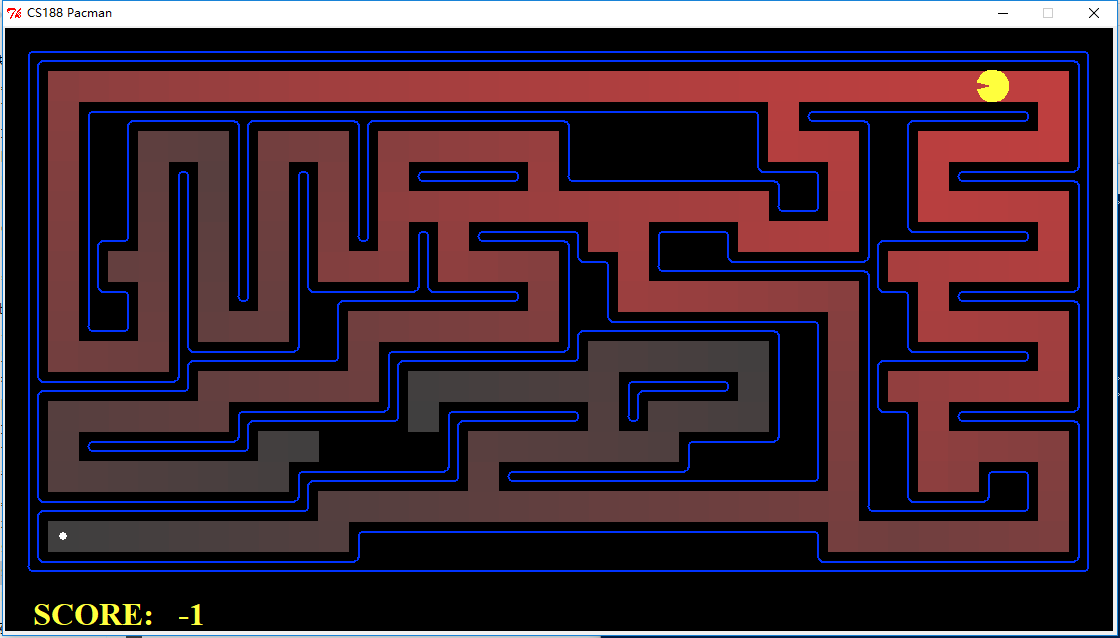
\includegraphics[width=15cm]{assets/Pacman}
\caption{Searching by BFS or DFS}
\end{figure}

\section{Code Framework}
There are several code fragments that can be shared among different search algorithms such as BFS, DFS and A*, e.g., code of file-reading, setting characters, printing results and so on.

\begin{lstlisting}[title=settings.py]
# -*- coding: utf-8 -*-

filename = 'MazeData.txt'
wall_char = '%'
space_char = ' '
start_char = 'S'
end_char = 'E'
\end{lstlisting}

\begin{lstlisting}[title=main.py]
# -*- coding: utf-8 -*-
import numpy as np
from queue import Queue
from bfs import bfs
import settings


def makePath(maze_origin, prev, start, end):
    '''
    Make a path presented by list from the prev matrix given.
    '''
    path = []
    current = end
    while current != start:
        path.insert(0, current)  # insert at the head of the path
        current = prev[current[0]][current[1]]
    return path


def makeMazeWithPath(maze_origin, path):
    '''
    Draw the path into the maze.
    '''
    maze = maze_origin.copy()

    for i in range(len(path)-1):
        if path[i][0] + 1 == path[i+1][0]:
            maze[path[i]] = '↓'
        elif path[i][0] - 1 == path[i+1][0]:
            maze[path[i]] = '↑'
        elif path[i][1] - 1 == path[i+1][1]:
            maze[path[i]] = '←'
        elif path[i][1] + 1 == path[i+1][1]:
            maze[path[i]] = '→'
        else:
            exit('[-] Path Error!')

    return maze


if __name__ == '__main__':
    with open(settings.filename) as file:
        maze = []  # list of list
        for i, line in enumerate(file):
            line = line.strip()  # delete EOL
            start_col = line.find(settings.start_char)
            end_col = line.find(settings.end_char)
            if start_col != -1:
                start = (i, start_col)
            if end_col != -1:
                end = (i, end_col)
            maze.append(list(line))  # append current row
    maze = np.array(maze)  # convert to numpy 2D-array

    prev = bfs(maze, start, end)  # use bfs() or astar()
    path = makePath(maze, prev, start, end)

    # Print the length of the path
    print('[+] Steps:', len(path))
    # Print the path in a list of coordinates
    print('[+] Path (in coordinates):\n', path)
    # Print the figure of the maze and the path
    print('[+] Path (in figure):')
    maze_with_path = makeMazeWithPath(maze, path)
    for line in maze_with_path:
        print(''.join(line))
\end{lstlisting}

%-----------------------------------------------------
\section{Searching by BFS}
\subsection{Overview}

BFS, a.k.a Breadth-First Search, is the simplest of the graph search algorithms. It is a search algorithm categoried as uninformed search. Breadth First Search explores equally in all directions. This is an incredibly useful algorithm, not only for regular path finding, but also for procedural map generation, flow field pathfinding, distance maps, and other types of map analysis.\cite{redblobgames}

I use numpy arrays to store the maze (which is read from a text file), and use a list of coordinates to store the path. After finding the path successfully, the length of the path, the list of those coordinates and a figure with path presented by arrows inside the maze are printed.

\subsection{Code}
I didn't use a ``visited'' matrix. Instead, I change the corresponding point into wall\_char to show that the point has been visited.

\begin{lstlisting}[title=bfs.py]
# -*- coding: utf-8 -*-
from queue import Queue
import settings


def bfs(maze_origin, start, end):
    '''
    Find a path in the maze given using BFS.
    '''
    maze = maze_origin.copy()

    rows = len(maze)     # num of rows of the maze
    cols = len(maze[0])  # num of columns of the maze
    prev = [[(-1, -1) for j in range(cols)] for i in range(rows)]  # record the path

    frontier = Queue()
    frontier.put(start)

    while not frontier.empty():
        current = frontier.get()
        if current == end:  # have explored to the end
            break

        row = current[0]
        col = current[1]

        # up
        if row > 0 and maze[row-1][col] != settings.wall_char:
            frontier.put((row-1, col))
            maze[row-1][col] = settings.wall_char
            prev[row-1][col] = (row, col)

        # down
        if row < rows - 1 and maze[row+1][col] != settings.wall_char:
            frontier.put((row+1, col))
            maze[row+1][col] = settings.wall_char
            prev[row+1][col] = (row, col)

        # left
        if col > 0 and maze[row][col-1] != settings.wall_char:
            frontier.put((row, col-1))
            maze[row][col-1] = settings.wall_char
            prev[row][col-1] = (row, col)

        # right
        if col < cols - 1 and maze[row][col+1] != settings.wall_char:
            frontier.put((row, col+1))
            maze[row][col+1] = settings.wall_char
            prev[row][col+1] = (row, col)

    return prev
\end{lstlisting}

\subsection{Result}
\begin{figure}[ht]
\centering
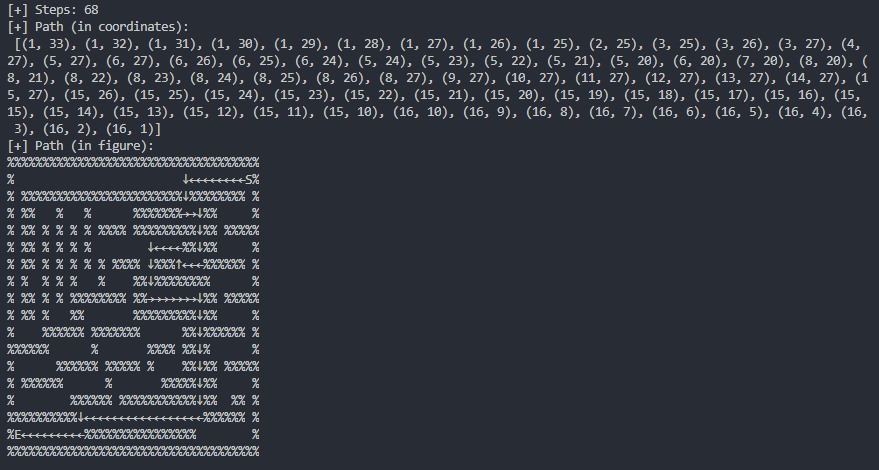
\includegraphics[width=15cm]{assets/result1.png}
\caption{Result of BFS}
\end{figure}

As shown in the figure above, the algorithm find a path of length 68. The path is printed as well.

%-----------------------------------------------------
\section{Discussion}
In this task, I use BFS to find a path from start point to end point in a given maze. BFS is simple and easy to understand, because we have learnt it in previous lessons. BFS satisfies optimality because of three facts:
\begin{itemize}
\item All shorter paths are expanded before any longer path;
\item There are finitely many paths of a certain length;
\item Eventually we must examine all paths of length d, and thus find the shortest solution.
\end{itemize}

However, there exist more powerful algorithms, such as A*, which I will study in the near future.

This is the first time that I have written a report in \LaTeX, and I am happy to learn a new tool that will be very useful in future.

%-----------------------------------------------------
\begin{thebibliography}{9}
\bibitem{redblobgames} 
Introduction to the A* Algorithm,
\\\texttt{https://www.redblobgames.com/pathfinding/a-star/introduction.html}
\end{thebibliography}

\end{document}